\section{The Chain Rule} \label{S:10.5.Chain_Rule}

\vspace*{-14 pt}
\framebox{\hspace*{3 pt}
\parbox{6.25 in}{\begin{goals}
\item What is the Chain Rule and how do we use it to
  find a derivative?  
\item How can we use a tree diagram to guide us in applying the Chain
  Rule? 
\end{goals}} \hspace*{3 pt}}


\subsection*{Introduction}

In single-variable calculus, we encountered situations in
which some quantity $z$ depends on $y$ and, in turn, $y$ depends on
$x$.  A change in $x$ produces a change in $y$, which consequently
produces a change in $z$.  Using the language of differentials that we saw
in the previous section, these changes are naturally related by
$$
dz = \frac{dz}{dy}~dy 
\hspace*{20pt}
\mbox{and}
\hspace*{20pt}
dy = \frac{dy}{dx}~dx.
$$
In terms of instantaneous rates of change, we then have
$$
dz = \frac{dz}{dy}\frac{dy}{dx}~dx = \frac{dz}{dx}~dx
$$
and thus
$$
\frac{dz}{dx} = \frac{dz}{dy}\frac{dy}{dx}.
$$
This most recent equation we call the {\em Chain Rule}.

In the case of a function $f$ of two variables where $z = f(x,y)$, it might be that both $x$ and $y$ depend on another variable $t$. A change in $t$ then produces changes in both $x$ and $y$, which then cause $z$ to change. In this section we will see how to find the change in $z$ that is caused by a change in $t$, leading us to multivariable versions of the Chain Rule involving both regular and partial derivatives. 

\begin{pa} \label{PA:10.5} Suppose you are driving around in the
  $x$-$y$ plane in such a way that your position at time $t$ is given by the vector-valued
  function 
  $$
  \vr(t) = \langle x(t), y(t) \rangle = \langle 2-t^2, t^3 + 1\rangle.
  $$
  The path taken is shown on the left of Figure
  \ref{F:10.5.preview}.  

  \begin{figure}
    \begin{center}
      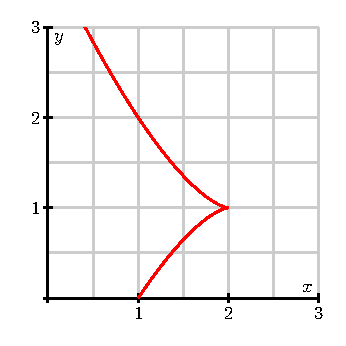
\includegraphics{figures/fig_10_5_preview_r.eps}
      \hspace*{20pt}
      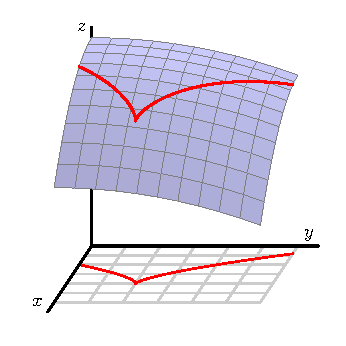
\includegraphics{figures/fig_10_5_preview_h.eps}
    \end{center}
    \caption{At left, your position in the plane; at right, the corresponding temperature.}
    \label{F:10.5.preview}
  \end{figure}
  Suppose, furthermore, that
  the temperature at a point in the plane is given by
  $$
  T(x,y) = 10 - \frac12x^2 -\frac15y^2,
  $$
  and note that the surface generated by $T$ is shown on the right of Figure \ref{F:10.5.preview}.  Therefore, as
  time passes, your position $(x(t), y(t))$ changes, and, as your position
  changes, the temperature $T(x,y)$ also changes.
  
  \ba
%\item What is your position at time $t=1$;  that is, what are the $x$-
 % and $y$-coordinates of your location?
%\item What is the temperature at this point?
\item The position function $\vr$ provides a parameterization $x = x(t)$ and $y = y(t)$ of the position at time $t$. By substituting $x(t)$ for $x$ and $y(t)$ for $y$ in the formula for $T$, we can write $T = T(x(t), y(t))$ as a function of $t$. Make these substitutions to write $T$ as a function of $t$ and then use the Chain Rule from single variable calculus to find $\frac{dT}{dt}$. (Do not do any algebra to simplify the derivative, either before taking the derivative, nor after.)
\item Now we want to understand how the result from part (a) can be obtained from $T$ as a multivariable function.  Recall from the previous section that small changes in $x$ and $y$ produce a change in $T$ that is approximated by 
\[\Delta T \approx  T_x\Delta x + T_y\Delta y.\]
The Chain Rule tells us about the instantaneous rate of change of $T$, and this can be found as  
\begin{equation} \label{eq:PA_10_5_1}
\lim_{\Delta t \to 0} \frac{\Delta T}{\Delta t} = \lim_{\Delta t \to 0} \frac{T_x \Delta x + T_y \Delta y}{\Delta t}.
\end{equation}
Use equation (\ref{eq:PA_10_5_1}) to explain why the instantaneous rate of change of $T$ that results from a change in $t$ is 
\begin{equation} \label{eq:PA_10_5_2}
\frac{dT}{dt} = \frac{\partial T}{\partial x} \frac{dx}{dt} + \frac{\partial T}{\partial y} \frac{dy}{dt}.
\end{equation} 
	\item  Using the original formulas for $T$, $x$, and $y$ in the problem statement, calculate all of the derivatives in Equation (\ref{eq:PA_10_5_2}) (with $T_x$ and $T_y$ in terms of $x$ and $y$, and $x'$ and $y'$ in terms of $t$), and hence write the right-hand side of Equation (\ref{eq:PA_10_5_2}) in terms of $x$, $y$, and $t$. 
	\item Compare the results of parts (a) and (c). Write a couple of sentences that identify specifically how each term in (c) relates to a corresponding terms in  (a). This connection between parts (a) and (c) provides a multivariable version of the Chain Rule. 
  \ea

\end{pa} 

\begin{activitySolution} 
  \ba
\item With $x(t) = 2-t^2$ and $y(t) = t^3+1$ we have 
\[T(x(t),y(t)) = 10-\frac{1}{2}\left(2-t^2\right)^2-\frac{1}{5}\left(t^3+1\right)^2.\]
So 
\[\frac{dT}{dt} = -\frac{1}{2}(2)\left(2-t^2\right)(-2t)-\frac{1}{5}(2)\left(t^3+1\right)(3t^2).\]

\item Since $\lim_{\Delta t \to 0} \frac{\Delta T}{\Delta t} = \frac{dT}{dt}$ and $T_x$ and $T_y$ don't depend on $\Delta t$, we have 
\begin{align*}
\lim_{\Delta t \to 0} \frac{T_x \Delta x + T_y \Delta y}{\Delta t} &= T_x \lim_{\Delta t \to 0} \frac{\Delta x}{\Delta t} + T_y  \lim_{\Delta t \to 0} \frac{\Delta y}{\Delta t} \\
	&= T_x \frac{dx}{dt} + T_y \frac{dy}{dt} \\
	&= \frac{\partial T}{\partial x} \frac{dx}{dt} + \frac{\partial T}{\partial y} \frac{dy}{dt}.
\end{align*}

	\item  Straightforward calculations show that 
\[T_x(x,y) = -x, \ T_y(x,y) = -\frac{2}{5}y, \ \frac{dx}{dt} = -2t, \ \text{ and } \ \frac{dy}{dt} = 3t^2.\]
Then
\begin{align*}
\frac{dT}{dt} &= \frac{\partial T}{\partial x} \frac{dx}{dt} + \frac{\partial T}{\partial y} \frac{dy}{dt} \\
	&= (-x)(-2t) - \frac{2}{5}y(3t^2).
\end{align*}
	
	\item With $x=2-t^2$ and $y = t^3+1$, the results of parts (a) and (c) are the same. The terms $-x$ and $-\frac{2}{5}y$ in (c) agree with what we get when we differentiate the outermost functions in (a). We can see where the terms $-2t$ and $3t^2$ in part (c) come from using the Chain Rule in (a) when we differentiate the innermost functions. 
  \ea
\end{activitySolution}

\afterpa 

\subsection*{The Chain Rule}

As Preview Activity \ref{PA:10.3} suggests, the following version of the Chain Rule holds in general.

\vspace*{5pt}
\nin \framebox{\hspace*{3 pt}
\parbox{6.25 in}{Let $z = f(x,y)$, where $f$ is a differentiable function of the independent variables $x$ and $y$, and let $x$ and $y$ each be differentiable functions of an independent variable $t$. Then
\begin{equation} \label{E:10.5.chain.rule}
\frac{dz}{dt} = \frac{\partial z}{\partial x} \frac{dx}{dt} + \frac{\partial z}{\partial y} \frac{dy}{dt}.
\end{equation}
} \hspace*{3 pt}}
\vspace*{5pt}

It is important to note the differences among the derivatives in (\ref{E:10.5.chain.rule}). Since $z$ is a function of the two variables $x$ and $y$, the derivatives in the Chain Rule for $z$ with respect to $x$ and $y$ are partial derivatives. However, since $x = x(t)$ and $y = y(t)$ are functions of the single variable $t$, their derivatives are the standard derivatives of functions of one variable. When we compose $z$ with $x(t)$ and $y(t)$, we then have $z$ as a function of the single variable $t$, making the derivative of $z$ with respect to $t$ a standard derivative from single variable calculus as well.

To understand why this Chain Rule works in general, suppose that some quantity $z$ depends on $x$ and $y$ so
that
\begin{equation}
  dz = \frac{\partial z}{\partial x}~dx + \frac{\partial z}{\partial
    y}~dy.
  \label{E:10.5.1}
\end{equation}
Next, suppose that $x$ and $y$ each depend on another quantity $t$, so that
\begin{equation}
  dx = \frac{dx}{dt}~dt
  \hspace*{20pt}
  \mbox{and}
  \hspace*{20pt}
  dy = \frac{dy}{dt}~dt.
  \label{E:10.5.2}
\end{equation}
    
Combining Equations~(\ref{E:10.5.1}) and (\ref{E:10.5.2}), we find that
$$
dz = \frac{\partial z}{\partial x}\frac{dx}{dt}~dt 
+ \frac{\partial z}{\partial y}\frac{dy}{dt}~dt = \frac{dz}{dt}~dt,
$$
which is the Chain Rule in this particular context, as expressed in Equation~\ref{E:10.5.chain.rule}.

\begin{activity} \label{PA:10.11} In the following questions, we apply the recently-developed Chain Rule in several different contexts.
  \ba
  \item Suppose that we have a function $z$ defined by $z(x,y) = x^2+xy^3$.  In addition, suppose that $x$ and $y$ are restricted to points that move around the plane by following
  a circle of radius $2$ centered at the origin that is parameterized by
    $$
    x(t) = 2\cos t,
    \hspace*{20pt}
    \mbox{and}
    \hspace*{20pt}
    y(t) = 2\sin t.
    $$
%    \begin{itemize}
%    \item What is the position when $t=\pi/4$?
%    \item What are the partial derivatives $\frac{\partial z}{
 %       \partial x}$ and $\frac{\partial z}{\partial y}$ at this
%      point? 
    Use the Chain Rule to find the resulting instantaneous rate of change $\frac{dz}{dt}$.  
%    \end{itemize}
      
  \item Suppose that the temperature on a metal plate is given by
    the function $T$ with 
    $$
    T(x,y) = 100-(x^2 + 4y^2),
    $$
    where the temperature is measured in degrees Fahrenheit
    and $x$ and $y$ are each measured in feet. 
    
    \begin{enumerate}[i.]
    \item Find $T_x$ and $T_y$.  What are the units on these partial
      derivatives?    
    \item Suppose an ant is walking along the $x$-axis at the rate
      of 2 feet per minute toward the origin.  When the ant is at
      the point $(2,0)$, what is the
      instantaneous rate of change in the temperature $dT/dt$ that
      the ant experiences.  Include units on
      your response.
    \item Suppose instead that the ant walks along an ellipse
      with $x = 6\cos(t)$ and $y = 3\sin(t)$, where
      $t$ is measured in minutes.  Find $\frac{dT}{dt}$ at
      $t = \pi/6$, $t=\pi/4$, and $t = \pi/3$.  What does this
      seem to tell you about the path along which the ant is
      walking?
    \end{enumerate}


  \item Suppose that you are walking along a surface whose elevation is given by a function $f$.  Furthermore, suppose that if you consider how your location corresponds to points in the $x$-$y$ plane, you know that when you pass the point $(2,1)$, your velocity vector is $\vv=\langle -1,2\rangle$.  If some contours of the function $f(x,y)$ are as
    shown in Figure \ref{F:10.5.contour}, estimate the rate of change
    $df/dt$ when you pass through $(2,1)$.

    \begin{figure}[ht]
      \begin{center}
        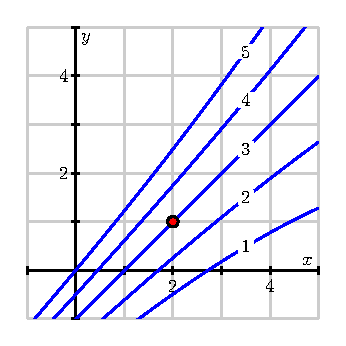
\includegraphics{figures/fig_10_3_activity_contour.eps}
      \end{center}
      \caption{Some contours of $f(x,y)$.}
      \label{F:10.5.contour}
    \end{figure}



  \ea

\end{activity} 

\begin{activitySolution}
\ba
\item According to the Chain Rule we have 
\begin{align*}
\frac{dz}{dt} &= \frac{\partial z}{\partial x} \frac{dx}{dt} + \frac{\partial z}{\partial y} \frac{dy}{dt} \\
	&= (2x+y^3)(-2\sin(t)) + (3xy^2)(2\cos(t)) \\
	&= -2(2\cos(t)+8\sin^3(t))\sin(t) + 48 \cos^2(t)\sin^2(t).
\end{align*}

\item 
	\begin{enumerate}[i.]
	\item We have
\begin{align*}
T_x(x,y) &= -2x \\
T_y(x,y) &= -8y,
\end{align*}
both measured in units of degrees Fahrenheit per foot. 
	\item In this situation we have $\frac{dx}{dt} = 2$ and $\frac{dy}{dt} = 0$. So 
\[\frac{dT}{dt} = -2x(2) -8y(0) = -4x.\]
Therefore, 
\[\frac{dT}{dt}\biggm|_{(2,0)} = -8 \frac{^{\circ}F}{\text{min}}.\]
	\item In this case we have 
\begin{align*}
\frac{dT}{dt} &= \frac{\partial T}{\partial x} \frac{dx}{dt} + \frac{\partial T}{\partial y} \frac{dy}{dt} \\	
	&= (-2x)(-6\sin(t)) - (8y)(3\cos(t)) \\
	&= 72\cos(t)\sin(t) - 72 \sin(t)\cos(t) \\
	&= 0.
\end{align*}
So
\[\frac{dT}{dt}\biggm|_{t=\pi/6} = 0 = \frac{dT}{dt}\biggm|_{t=\pi/4} =\frac{dT}{dt}\biggm|_{t=\pi/3}.\]
The fact that $\frac{dT}{dt} = 0$ means that $T$ is not changing, so on the path the ant is walking the temperature is constant. Note that 
\[T(6\cos(t), 3\sin(t)) = 100 - (36\cos^2(t) + 36\sin^2(t)) = 100-36 = 64,\]
so the ant is walking along a path of constant temperature $64^{\circ}F$. 
	\end{enumerate}
\item Since 
\[\frac{df}{dt}= \frac{\partial f}{\partial x} \frac{dx}{dt} + \frac{\partial f}{\partial y} \frac{dy}{dt},\]
we need to estimate $\frac{\partial f}{\partial x}$ and $\frac{\partial f}{\partial y}$ at $(2,1)$. Now
\begin{align*}
f_x(2,1) &\approx \frac{f(3,1) - f(1,1)}{2} \approx \frac{1.9-4.8}{2} = -1.45 \\
f_y(2,1) &\approx \frac{f(2,2) - f(2,0)}{2} \approx \frac{4.4-1.8}{2} = 1.3.
\end{align*}
The velocity vector at the point $(2,1)$ tells us $\frac{dx}{dt}$ and $\frac{dy}{dt}$ at the point $(2,1)$, so 
\[\frac{df}{dt}\biggm|_{(2,1)} \approx -1.45(-1) + 1.3(2) = 4.05.\]

\ea
\end{activitySolution}
\afterpa 

\subsection*{Tree Diagrams}

Up to this point, we have applied the Chain Rule to situations where
we have a function $z$ of variables $x$ and $y$, with both $x$ and $y$ depending on another single
quantity $t$.  We may apply the Chain Rule, however, when $x$ and $y$ each
depend on more than one quantity, or when $z$ is a function of more than two variables. It can be challenging to keep track
of all the dependencies among the variables, and thus a tree diagram can be a useful tool to organize our work. 
For example, suppose that $z$ depends on $x$ and $y$, and $x$ and $y$
both depend on $t$.  We may represent these relationships using the tree
diagram shown at left Figure \ref{F:10.5.tree.1}.  We place the dependent
variable at the top of the tree and connect it to the variables on
which it depends one level below.  We then connect each of those variables to the variable on which each depends.

\begin{figure}[ht]
  \begin{center}
    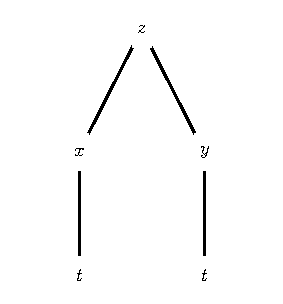
\includegraphics{figures/fig_10_5_tree_3.eps} \hspace{0.5in} 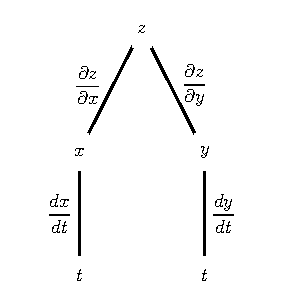
\includegraphics{figures/fig_10_5_tree_1.eps}
  \end{center}
  \caption{A tree diagram illustrating dependencies.}
  \label{F:10.5.tree.1}
\end{figure}

To represent the Chain Rule, we label every edge of the diagram with the
appropriate derivative or partial derivative, as seen at right in Figure
\ref{F:10.5.tree.1}.  To calculate an overall derivative according to the Chain Rule, we
construct the product of the derivatives along all paths connecting
the variables and then add all of these products.
For example, the
diagram at right in \ref{F:10.5.tree.1} illustrates the Chain Rule
$$
\frac{dz}{dt} = \frac{\partial z}{\partial x}\frac{dx}{dt} +
\frac{\partial z}{\partial y}\frac{dy}{dt}.
$$

%\begin{figure}[ht]
%  \begin{center}
%    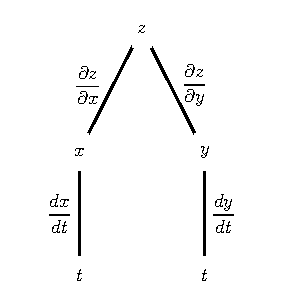
\includegraphics{figures/fig_10_5_tree_1.eps}
%  \end{center}
%  \caption{A tree diagram illustrating dependencies.}
%  \label{F:10.5.tree.1}
%\end{figure}

%\begin{activity} \label{PA:10.12} 
  \ba
  \item Suppose that $z=x^2 - 2xy^2$ and we would like to consider $x$
    and $y$ as expressed in polar coordinates:
    \begin{align*}
      x&=r\cos\theta \\
      y&=r\sin\theta \\
    \end{align*}
    \begin{itemize}
      \item If $r = 3$ and $\theta=\pi/6$, find $x$ and $y$.
      \item Use the Chain Rule to find the partial derivatives
        $$
        \frac{\partial z}{\partial r}
        \hspace*{20pt}
        \mbox{and}
        \hspace*{20pt}
        \frac{\partial z}{\partial \theta}
        $$
        at this point.
    \end{itemize}
      
  \item Consider the function $z = u^2 - v^2$ and suppose that
    \begin{align*}
      u & = e^x\cos y \\
      v & = e^x\sin y
    \end{align*}
    
    \begin{itemize}
      \item Find $u$ and $v$ if $x=0$ and $y=2\pi/3$.
      \item Use the Chain Rule to find the partial derivatives
        $$
        \frac{\partial z}{\partial x}
        \hspace*{20pt}
        \mbox{and}
        \hspace*{20pt}
        \frac{\partial z}{\partial y}
        $$
        at this point.
    \end{itemize}
      


  \ea

\end{activity} 
\afterpa 

%\begin{activity} \label{PA:10.12} 
  \ba
  \item Suppose that $z=x^2 - 2xy^2$ and we would like to consider $x$
    and $y$ as expressed in polar coordinates:
    \begin{align*}
      x&=r\cos\theta \\
      y&=r\sin\theta \\
    \end{align*}
    \begin{itemize}
      \item If $r = 3$ and $\theta=\pi/6$, find $x$ and $y$.
      \item Use the Chain Rule to find the partial derivatives
        $$
        \frac{\partial z}{\partial r}
        \hspace*{20pt}
        \mbox{and}
        \hspace*{20pt}
        \frac{\partial z}{\partial \theta}
        $$
        at this point.
    \end{itemize}
      
  \item Consider the function $z = u^2 - v^2$ and suppose that
    \begin{align*}
      u & = e^x\cos y \\
      v & = e^x\sin y
    \end{align*}
    
    \begin{itemize}
      \item Find $u$ and $v$ if $x=0$ and $y=2\pi/3$.
      \item Use the Chain Rule to find the partial derivatives
        $$
        \frac{\partial z}{\partial x}
        \hspace*{20pt}
        \mbox{and}
        \hspace*{20pt}
        \frac{\partial z}{\partial y}
        $$
        at this point.
    \end{itemize}
      


  \ea

\end{activity} 
\afterpa 

\begin{activity} \label{PA:10.13} 
\ba
\item Figure \ref{F:10.5.tree.2} shows the tree diagram we construct when (a) $z$ depends on $w$, $x$, and $y$, (b) $w$, $x$, and $y$ each depend on $u$ and $v$, and (c) $u$ and $v$ depend on $t$.

\begin{figure}[ht]
  \begin{center}
    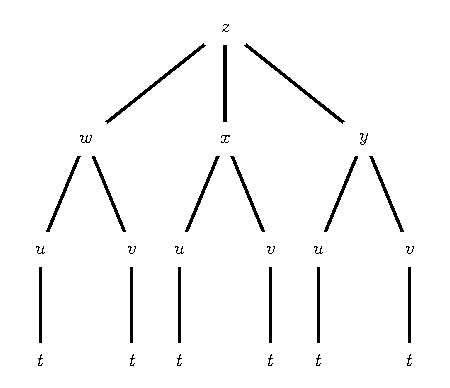
\includegraphics{figures/fig_10_5_tree_2.eps}
  \end{center}
  \caption{Three levels of dependencies}
  \label{F:10.5.tree.2}
\end{figure}

\begin{enumerate}[i.]
  \item Label the edges with the appropriate derivatives.
  \item Use the Chain Rule to write $\ds\frac{dz}{dt}$.
\end{enumerate}

\item Suppose that $z=x^2 - 2xy^2$ and that 
    \begin{align*}
      x&=r\cos\theta \\
      y&=r\sin\theta.
    \end{align*}
    \begin{enumerate}[i.]
	\item Construct a tree diagram representing the dependencies of $z$ on $x$ and $y$ and $x$ and $y$ on $r$ and $\theta$. 
	\item Use the tree diagram to find $\frac{\partial z}{\partial r}$. 
	\item Now suppose that $r = 3$ and $\theta=\pi/6$. Find the values of $x$ and $y$ that correspond to these given values of $r$ and $\theta$, and then use the Chain Rule to find the value of the partial derivative $\frac{\partial z}{\partial \theta}|_{(3,\frac{\pi}{6})}$.
    \end{enumerate}
    
  \ea

\end{activity} 

\begin{activitySolution}
\ba
\item 
	\begin{enumerate}[i.]
	\item A labeled tree diagram is shown here.
\begin{center}
\setlength{\unitlength}{1.5cm}
\begin{picture}(5,3.1)
\put(2,3){$z$}
\put(0.5,2){$w$}
\put(2,2){$x$}
\put(3.5,2){$y$}
\put(0,1){$u$}
\put(1,1){$v$}
\put(1.5,1){$u$}
\put(2.5,1){$v$}
\put(3,1){$u$}
\put(4,1){$v$}
\put(0,0){$t$}
\put(1,0){$t$}
\put(1.5,0){$t$}
\put(2.5,0){$t$}
\put(3,0){$t$}
\put(4,0){$t$}
\put(0.05,0.25){\line(0,1){0.65}}
\put(1.05,0.25){\line(0,1){0.65}}
\put(1.55,0.25){\line(0,1){0.65}}
\put(2.55,0.25){\line(0,1){0.65}}
\put(3.05,0.25){\line(0,1){0.65}}
\put(4.05,0.25){\line(0,1){0.65}}
\put(0.1,1.2){\line(3,5){0.4}}
\put(1,1.2){\line(-3,5){0.4}}
\put(1.6,1.2){\line(3,5){0.4}}
\put(2.5,1.2){\line(-3,5){0.4}}
\put(3.1,1.2){\line(3,5){0.4}}
\put(4,1.2){\line(-3,5){0.4}}
\put(0.75,2.25){\line(3,2){1}}
\put(2.075,2.25){\line(0,1){0.65}}
\put(3.25,2.25){\line(-3,2){1}}
\put(-0.25,0.5){$\frac{du}{dt}$}
\put(0.75,0.5){$\frac{dv}{dt}$}
\put(1.25,0.5){$\frac{du}{dt}$}
\put(2.25,0.5){$\frac{dv}{dt}$}
\put(2.75,0.5){$\frac{du}{dt}$}
\put(3.75,0.5){$\frac{dv}{dt}$}
\put(-0.1,1.5){$\frac{\partial w}{\partial u}$}
\put(0.9,1.5){$\frac{\partial w}{\partial v}$}
\put(1.4,1.5){$\frac{\partial x}{\partial u}$}
\put(2.4,1.5){$\frac{\partial x}{\partial v}$}
\put(2.9,1.5){$\frac{\partial y}{\partial u}$}
\put(3.9,1.5){$\frac{\partial y}{\partial v}$}
\put(0.85,2.65){$\frac{\partial z}{\partial w}$}
\put(1.75,2.5){$\frac{\partial z}{\partial x}$}
\put(2.85,2.65){$\frac{\partial z}{\partial y}$}
\end{picture}
\end{center}

	\item According to the Chain Rule we have 
\[\frac{dz}{dt} = \frac{\partial z}{\partial w}\frac{\partial w}{\partial u}\frac{du}{dt} + \frac{\partial z}{\partial w}\frac{\partial w}{\partial v}\frac{dv}{dt} + \frac{\partial z}{\partial x}\frac{\partial x}{\partial u}\frac{du}{dt} + \frac{\partial z}{\partial x}\frac{\partial x}{\partial v}\frac{dv}{dt} + \frac{\partial z}{\partial y}\frac{\partial y}{\partial u}\frac{du}{dt} + \frac{\partial z}{\partial y}\frac{\partial y}{\partial v}\frac{dv}{dt}.\]
	\end{enumerate}
\item 
	\begin{enumerate}[i.]
	\item A tree diagram is shown here.
\begin{center}
\setlength{\unitlength}{1.0cm}
\begin{picture}(2.5,3.5)
\put(-0.9,0.5){$r$} %Under x
\put(-0.65,0.85){\line(2,3){0.6}}
\put(0.7,0.5){$\theta$}
\put(0.65,0.85){\line(-2,3){0.6}}
\put(1.1,0.5){$r$} %Under y
\put(1.35,0.85){\line(2,3){0.6}}
\put(2.7,0.5){$\theta$}
\put(2.65,0.85){\line(-2,3){0.6}}
\put(0,2){$x$}
\put(-0.85,1.3){$\frac{\partial x}{\partial r}$}
\put(2,2){$y$}
\put(2.45,1.3){$\frac{\partial y}{\partial \theta}$}
\put(0.5,1.3){$\frac{\partial x}{\partial \theta}$}
\put(1.2,1.3){$\frac{\partial y}{\partial r}$}
\put(1,3.5){$z$}
\put(0.25,2.35){\line(2,3){0.6}}
\put(0.0,2.9){$\frac{\partial z}{\partial x}$}
\put(1.75,2.35){\line(-2,3){0.6}}
\put(1.6,2.9){$\frac{\partial z}{\partial y}$}
\end{picture}
\end{center}
	\item By the Chain Rule we have 
\[\frac{\partial z}{\partial r} = \frac{\partial z}{\partial x}\frac{\partial x}{\partial r} + \frac{\partial z}{\partial y}\frac{\partial y}{\partial r}.\]
	\item First note that $x(3,\pi/6) = 3\frac{\sqrt{3}}{2}$ and $y(3,\pi/6) = \frac{3}{2}$. Given that $z_x = 2x-2y^2$ and $z_y = -4xy$ we have $z_x(3, \pi/6)=3\sqrt{3}-3$ and $z_y(3,\pi/6) = -9\sqrt{3}$. Also, $x_r=\cos(\theta)$ and $y_r = \sin(\theta)$, so $x_r(3,\pi/6) = \frac{\sqrt{3}}{2}$ and $y_r(3,\pi/6) = \frac{1}{2}$. So  
\[\frac{\partial z}{\partial \theta}\bigm|_{(3,\frac{\pi}{6})} = (3\sqrt{3}-3)\left(\frac{\sqrt{3}}{2}\right) - 9\sqrt{3}\left(\frac{1}{2}\right).\]
	
	\end{enumerate}

\ea
\end{activitySolution}

\afterpa 





\begin{summary}
\item The Chain Rule is a tool for differentiating a composite for
  functions.  In its simplest form, it says that if $f(x,y)$ is a
  function of two variables and $x(t)$ and $y(t)$ depend on $t$, then
  $$
  \frac{df}{dt} = \frac{\partial f}{\partial x}\frac{dx}{dt}
  + \frac{\partial f}{\partial y}\frac{dy}{dt}.
  $$

\item A tree diagram can be used to represent the dependence of variables on other variables. By following the links in the tree diagram, we can form chains of partial derivatives or derivatives that can be combined to give a desired partial derivative. 
\end{summary}




\nin \hrulefill

\begin{exercises} 

\item Find the indicated derivative.  In each case, state the version of the Chain Rule that you are using.
	\ba	
	\item $\frac{df}{dt}$, if $f(x,y) = 2x^2y$, $x=\cos(t)$, and $y=\ln(t)$.

	\item $\frac{\partial f}{\partial w}$, if $f(x,y) = 2x^2y$, $x=w+z^2$, and $y=\frac{2z+1}{w}$



	\item $\frac{\partial f}{\partial v}$, if $f(x,y,z) = 2x^2y+z^3$, $x=u-v+2w$, $y=w2^v-u^3$, and $z = u^2-v$
	\ea

\begin{exerciseSolution}
\ba 
\item The chain rule says that
\begin{align*}
\frac{df}{dt} &= \frac{\partial f}{\partial x}\frac{dx}{dt} + \frac{\partial f}{\partial y}\frac{dy}{dt} \\
	&= (4xy)\left(-\sin(t)\right) + (2x^2)\left(\frac{1}{t}\right) \\
	&= -4 \cos(t) \sin(t) \ln(t) + \frac{2\cos^2(t)}{t}.
\end{align*}
\item By the chain rule we have
\begin{align*}
\frac{\partial f}{\partial w} &= \frac{\partial f}{\partial x} \frac{\partial x}{\partial w}+ \frac{\partial f}{\partial y} \frac{\partial y}{\partial w} \\
	&= \left( 4xy \right)\left( 1 \right) + \left( 2x^2 \right)\left( -\frac{2z+1}{w^2} \right) \\
	&= \left( \frac{(2z+1)4(w+z^2)y}{w} \right) - \left( \frac{2(2z+1)((w+z^2)^2}{w^2} \right).
\end{align*}

\item By the chain rule we have
\begin{align*}
\frac{\partial f}{\partial v} &= \frac{\partial f}{\partial x} \frac{\partial x}{\partial v}+ \frac{\partial f}{\partial y} \frac{\partial y}{\partial v} + \frac{\partial f}{\partial z} \frac{\partial z}{\partial v} \\
	&= \left( 4xy \right)\left( -1 \right) + \left( 2x^2 \right)\left( w^2 \right) + \left( 3z^2 \right)\left( -1 \right)  \\
	&= -4(u-v+2w)(w2^v-u^3) + 2(u-v+2w)^2w^2 - 3(u-v+2w)^2.
\end{align*}

\ea

\end{exerciseSolution}

\item Let $z = u^2 - v^2$ and suppose that
    \begin{align*}
      u & = e^x\cos y \\
      v & = e^x\sin y
    \end{align*}
    
    \ba
      \item Find the values of $u$ and $v$ that correspond to $x=0$ and $y=2\pi/3$.
      \item Use the Chain Rule to find the general partial derivatives
        $$
        \frac{\partial z}{\partial x}
        \hspace*{20pt}
        \mbox{and}
        \hspace*{20pt}
        \frac{\partial z}{\partial y}
        $$
        and then determine both $\frac{\partial z}{\partial x}\bigm|_{(0, \frac{2\pi}{3})}$ and $\frac{\partial z}{\partial y}\bigm|_{(0, \frac{2\pi}{3})}$.
     \ea

\begin{exerciseSolution}
    \ba
      \item Evaluating $u$ and $v$ at $x=0$ and $y=2\pi/3$ yields
\[u(0,2\pi/3) = \cos(2\pi/3) = -\frac{1}{2} \ \text{ and } \ v(0,2\pi/3) = \sin(2\pi/3) = \frac{\sqrt{3}}{2}.\]
      \item By the Chain Rule we have
\begin{align*}
\frac{\partial z}{\partial x} &= \frac{\partial z}{\partial u} \frac{\partial u}{\partial x} + \frac{\partial z}{\partial v} \frac{\partial v}{\partial x} \\
	&= 2ue^x\cos(y) -2ve^x \sin(y) \\
	&= 2e^{2x}\cos^2(y) - 2e^{2x}\sin^2(y)
\end{align*}
and
\begin{align*}
\frac{\partial z}{\partial y} &= \frac{\partial z}{\partial u} \frac{\partial u}{\partial y} + \frac{\partial z}{\partial v} \frac{\partial v}{\partial y} \\
	&= -2ue^x\sin(y) -2ve^x \cos(y) \\
	&= -2e^{2x}\cos(y)\sin(y) - 2e^{2x}\sin(y)\cos(y) \\
	&= -4e^{2x}\cos(y) \sin(y).
\end{align*}
Note that 
\[\frac{\partial z}{\partial x} = 2u^2-2v^2 \ \text{ and } \ \frac{\partial z}{\partial y} = -4uv,\]
so
\begin{align*}
\frac{\partial z}{\partial x}\biggm|_{(0, \frac{2\pi}{3})} &= 2\left(-\frac{1}{2}\right)^2 -2\left(\frac{\sqrt{3}}{2}\right)^2 = -1 \\
\frac{\partial z}{\partial y}\biggm|_{(0, \frac{2\pi}{3})} &= -4\left(-\frac{1}{2}\right)\left(\frac{\sqrt{3}}{2}\right) = \frac{2\sqrt{3}}{2}.
\end{align*}
     \ea
\end{exerciseSolution}
        
 \item Suppose that $T = x^2 + y^2 - 2z$ where
  \begin{align*}
    x & = \rho\sin\phi\cos\theta \\
    y & = \rho\sin\phi\sin\theta \\
    z & = \rho\cos\phi
  \end{align*}

  \ba
    \item Construct a tree diagram representing the dependencies among the variables.
    \item Apply the chain rule to find the partial derivatives
      $$
      \frac{\partial T}{\partial\rho},
      \frac{\partial T}{\partial\phi},
      \ 
      \mbox{and}
      \ 
      \frac{\partial T}{\partial\theta}.
      \hspace*{20pt}
      $$
    \ea

\begin{exerciseSolution}

  \ba
    \item A tree diagram that represents the dependencies among the variables is shown below.
\begin{center}
\setlength{\unitlength}{1.0cm}
\begin{picture}(7,5)
\put(0,0){$\rho$}
\put(1,0){$\phi$}
\put(2,0){$\theta$}

\put(2.5,0){$\rho$}
\put(3.5,0){$\phi$}
\put(4.5,0){$\theta$}

\put(5,0){$\rho$}
\put(6,0){$\phi$}
\put(7,0){$\theta$}

\put(1,2){$x$}
\put(3.5,2){$y$}
\put(6,2){$z$}

\put(3.5,4){$T$}

\put(0.2,0.35){\line(1,2){0.75}}
\put(1.1,0.35){\line(0,1){1.5}}
\put(2.0,0.35){\line(-1,2){0.75}}

\put(2.7,0.35){\line(1,2){0.75}}
\put(3.6,0.35){\line(0,1){1.5}}
\put(4.5,0.35){\line(-1,2){0.75}}

\put(5.2,0.35){\line(1,2){0.75}}
\put(6.1,0.35){\line(0,1){1.5}}
\put(7.0,0.35){\line(-1,2){0.75}}

\put(1.4,2.2){\line(5,4){2.0}}
\put(3.6,2.3){\line(0,1){1.5}}
\put(5.9,2.2){\line(-5,4){2.0}}
\end{picture}
\end{center}.

    \item By the Chain Rule we have 
\begin{align*}
\frac{\partial T}{\partial\rho} &= \frac{\partial T}{\partial x} \frac{\partial x}{\partial\rho} + \frac{\partial T}{\partial y} \frac{\partial y}{\partial\rho}  + \frac{\partial T}{\partial z} \frac{\partial z}{\partial\rho} \\
	&= 2x\sin(\phi) \cos(\theta) + 2y\sin(\phi) \sin(\theta) - 2\cos(\phi) \\
	&= 2\rho\sin^2(\phi) \cos^2(\theta) + 2\rho\sin^2(\phi) \sin^2(\theta) - 2\rho\cos^(\phi),
\end{align*}
\begin{align*}
\frac{\partial T}{\partial \phi} &= \frac{\partial T}{\partial x} \frac{\partial x}{\partial \phi} + \frac{\partial T}{\partial y} \frac{\partial y}{\partial \phi}  + \frac{\partial T}{\partial z} \frac{\partial z}{\partial \phi} \\
	&= 2x \rho \cos(\phi) \cos(\theta) + 2y \rho \cos(\phi) \sin(\theta) + 2\sin(\phi) \\
	&= 2\rho^2 \cos(\phi) \sin(\phi) \cos^2(\theta) + 2\rho^2 \cos(\phi) \sin(\phi) \sin^2(\theta) + 2\sin^(\phi),
\end{align*}
and
\begin{align*}
\frac{\partial T}{\partial \theta} &= \frac{\partial T}{\partial x} \frac{\partial x}{\partial \theta} + \frac{\partial T}{\partial y} \frac{\partial y}{\partial \theta}  + \frac{\partial T}{\partial z} \frac{\partial z}{\partial \theta} \\
	&= -2x \rho \sin(\phi) \sin(\theta) + 2y \rho \sin(\phi) \cos(\theta)  \\
	&= -2\rho^2 \sin^2(\phi) \cos(\theta) \sin(\theta) + 2\rho^2 \sin^2(\phi) \cos(\theta) \sin(\theta).
\end{align*}

    \ea
    

\end{exerciseSolution}
     
\item Suppose that the temperature on a metal plate is given by
    the function $T$ with 
    $$
    T(x,y) = 100-(x^2 + 4y^2),
    $$
    where the temperature is measured in degrees Fahrenheit
    and $x$ and $y$ are each measured in feet. 
    Now suppose that an ant is walking on the metal plate in such a way that it walks in a straight line from the point $(1,4)$ to the point $(5,6)$.
    \ba
    	\item Find parametric equations $(x(t),y(t))$ for the ant's coordinates as it walks the line from $(1,4)$ to $(5,6)$.
	\item What can you say about $\frac{dx}{dt}$ and $\frac{dy}{dt}$ for every value of $t$?
	\item Determine the instantaneous rate of change in temperature with respect to $t$ that the ant is experiencing at the moment it is halfway from $(1,4)$ to $(5,6)$, using your parametric equations for $x$ and $y$.  Include units on your answer.
    \ea    

\begin{exerciseSolution}
    \ba
    \item A direction vector for this line is $\langle 5-1, 6-4 \rangle = \langle 4, 2 \rangle$, so parametric equations $(x(t),y(t))$ for the ant's coordinates as it walks the line from $(1,4)$ to $(5,6)$ are
\[x(t) = 1 + 4t \ \text{ and } \ y(t) = 4 + 2t.\]

	\item Since $x$ and $y$ are linear functions of $t$, we see that $\frac{dx}{dt} = 4$ and $\frac{dy}{dt} = 2$ are both constant. 
	
	\item We want $\frac{dT}{dt}\bigm|_{t=1/2}$. The Chain Rule tells us that 
	\begin{align*}
	\frac{dT}{dt} &= \frac{\partial T}{\partial x} \frac{dx}{dt} + \frac{\partial T}{\partial y} \frac{dy}{dt} \\
		&= (-2x)(4) + (-8y)(2) \\
		&= -8(1 + 4t) - 16(4 + 2t).
	\end{align*}
	So
	\[\frac{dT}{dt}\biggm|_{t=1/2} = -8(3) - 16(5) = 104 \ \frac{^{\circ}\text{F}}{\text{ft}}.\]
		
    \ea  
\end{exerciseSolution}
     
\item There are several proposed formulas to approximate the surface
   area of the human body.
   One model\footnote{DuBois D, DuBois DF. A formula to
     estimate the approximate surface area if height and weight be
     known.  \emph{Arch Int Med} 1916;17:863-71.} uses the formula
   $$
    A(h,w) = 0.0072 h^{0.725}w^{0.425},
   $$
   where $A$ is the surface area in square meters, $h$ is the
   height in centimeters, and $w$ is the weight in kilograms.

   Since a person's height $h$ and weight $w$ change over time,
  $h$ and $w$ are functions of time
   $t$. Let us think about what is happening to a child whose height
  is $60$ centimeters and weight is $9$ kilograms. Suppose,
  furthermore, that 
  $h$ is increasing at an instantaneous rate of 20 centimeters per year and $w$ is
 increasing at an instantaneous rate of $5$ kg per year. 

 Determine the instantaneous rate at which the child's surface area is changing at this point in time.

\begin{exerciseSolution}
We want to find $\frac{dA}{dt}\bigm|_{(60,9)}$ given that $\frac{dh}{dt} = 20$ and $\frac{dw}{dt} = 5$. The Chain Rule tells us that 
\begin{align*}
\frac{dA}{dt} &= \frac{\partial A}{\partial h} \frac{dh}{dt} + \frac{\partial A}{\partial w} \frac{dw}{dt} \\
	&= 0.00522h^{-0.275}w^{0.425}(20) + 0.00306h^{0.725}w^{-0.575}(5).
\end{align*}
So
\[\frac{dA}{dt}\biggm|_{(60,9)} \approx 0.1703 \ \frac{\text{m}^2}{\text{yr}}.\]
\end{exerciseSolution}

\item Let $z = f(x,y) = 50 - (x+1)^2 - (y+3)^2$ and $z = h(x,y) = 24 - 2x - 6y$.

Suppose a person is walking on the surface $z = f(x,y)$ in such a way that she walks the curve which is the intersection of $f$ and $h$. 
	\ba
	\item Show that $x(t) = 4 \cos(t)$ and $y(t) = 4 \sin(t)$ is a parameterization of the ``shadow'' in the $x$-$y$ plane of the curve that is the intersection of the graphs of $f$ and $h$.

	\item Use the parameterization from part (a) to find the instantaneous rate at which her height is changing with respect to time at the instant $t = 2\pi/3$.  
	
	\ea

\begin{exerciseSolution}
	\ba
	\item Notice that $f(x,y) = h(x,y)$ when $50-x^2-2x-1-y^2-6y-9=24-2x-6y$ or when $x^2+y^2=16$. This is the circle centered at the origin of radius 4, which has a parameterization $x(t) = 4 \cos(t)$ and $y(t) = 4 \sin(t)$.  

	\item We want to find $\frac{df}{dt}\bigm|_{t=2\pi/3}$. The Chain Rule tells us that 
\begin{align*}
\frac{df}{dt} &= \frac{\partial f}{\partial x} \frac{dx}{dt} + \frac{\partial f}{\partial y} \frac{dy}{dt} \\
	&= (-2(x+1))(-4\sin(t)) + (-3(y+3)^2)(4\cos(t)).
\end{align*}
Now $x(2\pi/3) = -2$ and $y(2\pi/3) = 2\sqrt{3}$, so 
\[\frac{df}{dt}\biggm|_{t=2\pi/3} \approx 243.78.\]

	\ea

\end{exerciseSolution}

\item The voltage $V$ (in volts) across a circuit is given by Ohm's Law: $V = IR$, where $I$ is the current (in amps) in the circuit and $R$ is the resistance (in ohms). Suppose we connect two resistors with resistances $R_1$ and $R_2$ in parallel as shown in Figure \ref{F:10.5.CR_Circuit}. The total resistance $R$ in the circuit is then given by
\[\frac{1}{R} = \frac{1}{R_1} + \frac{1}{R_2}.\]
\begin{figure}[ht]
\begin{minipage}{4in}
        \ba
    \item Assume that the current, $I$, and the resistances, $R_1$ and $R_2$, are changing over time, $t$. Use the Chain Rule to write a formula for $\frac{dV}{dt}$.



    \item Suppose that, at some particular point in time, we measure the current to be 3 amps and that the current is increasing at $\frac{1}{10}$ amps per second, while resistance $R_1$ is 2 ohms and decreasing at the rate of 0.2 ohms per second and $R_2$ is 1 ohm and increasing at the rate of $0.5$ ohms per second. At what rate is the voltage changing at this point in time?



    \ea
\end{minipage} \hspace{0.2in}
\begin{minipage}{2.3in}
\begin{center}
%\resizebox{!}{1.15in}{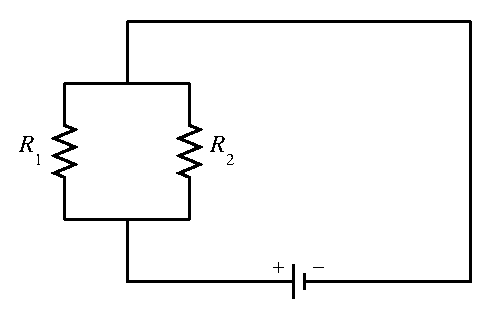
\includegraphics{10_5_CR_Circuit}}
 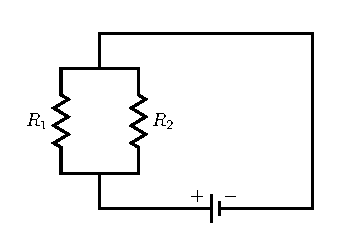
\includegraphics{figures/fig_10_5_resistors.eps}
\end{center}
\caption{Resistors in parallel.}
\label{F:10.5.CR_Circuit}
\end{minipage}
\end{figure}

\begin{exerciseSolution}
        \ba
    \item Given that $R = \frac{R_1R_2}{R_1+R_2}$ we have 
\[V(I,R_1,R_2) = \frac{IR_1R_2}{R_1+R_2}.\]
The Chain Rule tells us that 
\begin{align*}
\frac{dV}{dt} &= \frac{\partial V}{\partial I} \frac{dI}{dt} + \frac{\partial V}{\partial R_1} \frac{dR_1}{dt} + \frac{\partial V}{\partial R_2} \frac{dR_2}{dt} \\
	&=  \left(\frac{R_1R_2}{R_1+R_2}\right)\frac{dI}{dt} + \left(\frac{IR_2^2}{(R_1+R_2)^2}\right) \frac{dR_1}{dt} +  \left(\frac{IR_1^2}{(R_1+R_2)^2}\right) \frac{dR_2}{dt}.
\end{align*}


    \item Let $t_0$ be this time, then 
\[\frac{dV}{dt}\biggm|_{t=t_0} = \left(\frac{2}{3}\right)(0.1) + \left(\frac{1}{3}\right)(-0.2) + \left(\frac{4}{3}\right)(0.5) = \frac{2}{3} \ \frac{\text{V}}{\text{sec}}.\]




    \ea
\end{exerciseSolution}

\end{exercises}
\afterexercises


\clearpage
